\begin{figure*}[tb]
	\begin{minipage}[b]{.2\textwidth}
		\caption{Mbandaka-Gruppe: Typvertreter.\\1:~Taf.~32.6; 2:~Taf.~32.4; 3:~Taf.~28.4; 4:~Taf.~28.10; 5:~Taf.~30.3.}
		\label{fig:MBA_Typentafel}
	\end{minipage}\hfill
	\begin{minipage}[b]{.8\textwidth}
		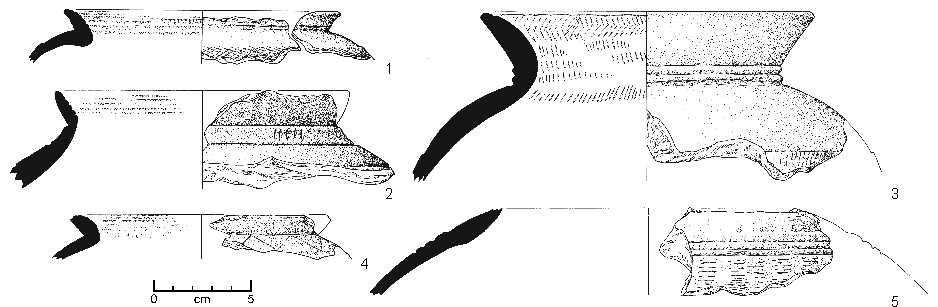
\includegraphics[width=\textwidth]{fig/MBA-Typen.pdf}
	\end{minipage}
\end{figure*}


\subsubsection{Mbandaka-Gruppe}\label{sec:MBA-Gr}

Keramik des ebenfalls aus dem Inneren Kongobecken bekannten Mbandaka-Stils findet sich, wie auch die etwa zeitgleiche Bondongo-Keramik (Kap.~\ref{sec:BDG-Gr}) ausnahmslos im äußersten Süden des Arbeitsgebietes. Zweifelsfrei der Stilgruppe zurechenbare Stücke sind ausschließlich an den 1987 am rechnen Ufer des Kongo erschlossenen Fundstellen (Fpl.~234--237) sowie in Bobusa (Fpl.~239) an der Einmündung des \mbox{Sangha} in den Kongo belegt (Abb.~\ref{fig:MBA_Verbreitung}). Neben 28 individuell aufgenommenen GE wurden zehn der Mbandaka-Gruppe zugewiesene Stücke summarisch aufgenommen. Im ersten Abtrag eines lediglich 1\,$\times$\,1\,m großen Testschnitts in Bobusa wurden zwei GE ausgegraben (Kat.-Nr.~6). Der Rest stammt aus Surveys von modernen Dorfflächen und weist eine starke Fragmentierung auf. Etwa 78\,\% aller GE der Mbandaka-Gruppe sind kleiner als 70\,$\times$\,70\,mm. Lediglich bei einer GE aus Maberu am Kongo (Fpl.~235) handelt es sich um ein hinreichend großes Fragment (Abb.~\ref{fig:MBA_Typentafel}.3). Dies hat zur Folge, dass zwar 14 GE als sicher der Mbandaka-Gruppe zugehörig angesprochen werden, weitere 14~GE jedoch nur unter Vorbehalt als Teil der Stilgruppe anzusehen oder nicht zweifelsfrei von anderen Stilgruppen wie Ngombe (Kap.~\ref{sec:NGO-Gr}) oder Bondongo (Kap.~\ref{sec:BDG-Gr}) abzugrenzen sind. Das Gros der Scherben der Mbandaka-Gruppe stammt von den beiden Fundstellen Lukolela (Fpl.~234) und Sungu (Fpl.~236) am rechten Ufer des Kongo, wenige Kilometer flussaufwärts von der Einmündung des \mbox{Sangha}. Das Inventar der Mbandaka-Gruppe aus dem Arbeitsgebiet setzt sich zu etwa gleichen Teilen aus Randscherben und Fragmenten der Gefäßwandung zusammen.


\paragraph{Technologische Merkmale}\hspace{-.5em}|\hspace{.5em}%
Die Keramik des Mbandaka-Stils zeichnet sich, wie auch alle der hauptsächlich aus dem Inneren Kongobecken bekannten Stilgruppen (Kap.~\ref{sec:InneresKongobeckenGruppen}), durch das fast vollständige Fehlen nichtplastischer Partikel im Scherben aus. \textit{Fabrics} des Typs 1 machen 95\,\% aller GE der Mbandaka-Gruppe aus. Lediglich zwei bei der Grabung BBS~87/1 in Bobusa am \mbox{Sangha} (Kat.-Nr.~6) gefundene GE des Mbandaka-Stils (Taf.~33.15) enthalten Fragmente zerstoßener Keramik und sind dem \textit{Fabric} 9 zuzuweisen. Diese Schamott-Magerung zeichnet sich durch Anteile zwischen 15--40\,\% und Partikeln aller Größenklassen bis einschließlich \textit{very coarse} (Tab.~\ref{tab:Keramik_PartikelGr}) aus. Die Färbung der Stücke deutet eine regelhafte Nutzung weißbrennender Tone für die Herstellung der Gefäße an. Hinweise auf die Nutzung rotbrennender Tone ergaben sich lediglich bei einer GE, während 43\,\% aller Scherben auf weißbrennende Tone hinweisen.

\begin{figure*}[p]
	\centering
	\includegraphics[width=\textwidth]{fig/MBA_Verbreitung.pdf}
	\caption{Mbandaka-Gruppe: Verbreitung im Arbeitsgebiet sowie im Inneren Kongobecken \parencite[grau nach][560--561 Karte 10]{Wotzka.1995}.}
	\label{fig:MBA_Verbreitung}
\end{figure*}


\paragraph{Formen}\hspace{-.5em}|\hspace{.5em}%
Bei insgesamt 26~GE der Mbandaka-Gruppe konnte die Gefäßform angesprochen werden, bei zehn dieser GE jedoch lediglich unter Vorbehalt. Die bestimmende Grundform sind Gefäße mit stark konvexer Wandung und kurzem, ausbiegendem Rand vom Typ D1/2 (81\,\%). Diese entsprechen dem von \textsc{Wotzka} (ebd. 139~Tab.~60) beschriebenen Gefäßtyp 67, der im Material aus dem Inneren Kongobecken mit 77,6\,\% das Inventar der Mbandaka-Gruppe ebenfalls deutlich dominiert. Im Arbeitsgebiet fanden sich jeweils nur einzelne Vertreter hoher Gefäße des Typs B1 sowie B4 und von Gefäßen mit leicht konvexer Wandung und ausgeprägtem Halsbereich des Typs C1/2. Bei keiner der GE aus dem Arbeitsgebiet ließ sich die Mündungshöhe rekonstruieren.\footnote{Lediglich die Durchmesser können als Indikatoren für Größe sowie Proportionen der Gefäße der Mbandaka-Gruppe herangezogen werden. Die maximalen Durchmesser der stark kugelbauchigen Gefäße des Typs D1/2 schwanken zwischen 15--28\,cm, während die Durchmesser der Gefäßmündungen bei 10,5--18\,cm liegen. Die minimalen Durchmesser am Übergang des Gefäßrandes zum -bauch liegen zwischen 5--14\,cm.} Die Ränder sind fast ausschließlich ausbiegend gestaltet, wobei kurze, gerade ausbiegende (B1.1; 38\,\%) sowie kurze, konkav ausbiegende Ränder (B2.1; 38\,\%) deutlich überwiegen. Die Mbandaka-Keramik des Inneren Kongobeckens wird durch ausbiegende, leicht verjüngende und innen gewölbte Ränder bestimmt, die \textsc{Wotzka} (ebd. 130, 140, 436 Taf.~2) als Typ R65 systematisiert und die in der für das nordwestliche Kongobecken erarbeiteten Systematik sowohl durch die Typen B1.1 als auch B2.1 repräsentiert sind (Tab.~\ref{tab:Keramik_RandFormen}).\footnote{\textsc{Wotzka} (1995: 436 Taf.2) fasst unter der Randform R65 gerade wie konkave ausbiegende Ränder zusammen. Während die ersten vier Varianten der Randform R65 der -- im Zuge dieser Arbeit verwendeten -- Randform B2.1 entsprechen (Tab.~\ref{tab:Keramik_RandFormen}), sind die beiden letzten Varianten als Randform B1.1 anzusehen.} Die Halspartien der Gefäße zeichnen sich, wenn sie dezidiert ausgearbeitet wurden, regelhaft durch kurze Kegelhälse aus (Abb.~\ref{fig:MBA_Typentafel}.2). Im Arbeitsgebiet konnte keine Bodenscherbe dem Mbandaka-Stil zugeordnet werden. Im angrenzenden Inneren Kongobecken lassen sich Angaben zur Ausgestaltung der Gefäßböden lediglich anhand von zwei GE machen. In einem Fall handelt es sich um einen runden Boden des Typs B1, während die zweite GE einen Omphalosboden (B7) aufweist (ebd. 140). 

\paragraph{Verzierungen}\hspace{-.5em}|\hspace{.5em}%
Die Mbandaka-Keramik weist ein stark eingeschränktes Spektrum an Verzierungselementen auf. Horizontale Rillen (Tab.~\ref{tab:Verzierungselemente}: 02.1) entsprechen etwa 56\,\% aller aufgenommen Verzierungselemente und finden sich vor allem an der Innenseite der Gefäßränder sowie außen im Hals- und Schulterbereich. Ebenfalls innenseitig am Rand sowie auf der Schulter sowie dem Gefäßbauch lässt sich teilweise \textit{banfwa-nfwa}-Verzierung (Tab.~\ref{tab:Verzierungselemente}: 08; 13\,\%) beobachten. Des Weiteren umfasst das Spektrum der Verzierungselemente der Mbandaka-Gruppe vereinzelte Varietäten von Ritzlinien (Tab.~\ref{tab:Verzierungselemente}: 01.2, 01.6, 01.8) oder Riefen (Tab.~\ref{tab:Verzierungselemente}: 02.2, 02.4--5) sowie Eindrücken (Tab.~\ref{tab:Verzierungselemente}: 04.12, 04.15, 04.17, 05.1). Verzierungen finden sich vornehmlich im Schulterbereich (35\,\%) sowie innenseitig am Rand (28\,\%). Auffällig ist, dass die Außenseite der Ränder fast nie verziert ist (4\,\%). Aufgrund der Erhaltung ließen sich keine Gefäßunterteile der Mbandaka-Gruppe identifizieren. Für das Fundgut aus dem nordwestlichen Kongobecken muss daher offenbleiben, wie die Verzierung der Bodenansätze oder Standflächen aussah. Gefäße der Mbandaka-Gruppe im benachbarten Inneren Kongobecken zeichnen sich ebenfalls regelhaft durch eingeritzte Motive sowie \textit{banfwa-nfwa}-Verzierung aus (ebd. 140). Auch innerhalb des Inventars aus dem Inneren Kongobecken sind Belege für Gefäßunterteile selten. Die wenigen vorliegenden Stücke zeigen flächiges \textit{banfwa-nfwa} sowie girlandenartige Ritzlinien auf den Unterseite (ebd. 141).


\paragraph{Datierung}\hspace{-.5em}|\hspace{.5em}%
Für keine der im Arbeitsgebiet der Mbandaka-Gruppe zugewiesenen GE liegt ein absoluter Datierungsansatz vor. Lediglich die beiden im ersten Abtrag der Grabung BBS 87/1 in Bobusa am unteren \mbox{Sangha} (Kat.-Nr.~6; Fpl.~239) aufgedeckten GE stammen aus einem stratifizierten Kontext.\footnote{Die Grabung erbrachte lediglich 67~GE und innerhalb der drei Funde führenden Schichten ergab sich keine deutliche Stilgruppenabfolge. Funde der Bobusa-Gruppe (Kap.~\ref{sec:BBS-Gr}) finden sich ebenfalls in allen Schichten (siehe Kat.-Nr.~6).} Für das Material aus dem Inneren Kongobecken konnte \textsc{Wotzka} (ebd. 142 Tab.~62, 143), auf Basis der Fundvergesellschaftungen in drei Grabungsbefunden, eine chronologische Ansprache der Mbandaka-Keramik erarbeiten. Die Grabung MBA 81/2 erbrachte ein mit Mbandaka-Keramik vergesellschaftetes Radiokohlenstoffdatum, dass das späte \mbox{12.--14.~Jh.} n.~Chr. abdeckt (ebd. 138; 305--308). Abschließend sieht \textsc{Wotzka} (ebd. 143) für die Mbandaka-Gruppe \enquote{eine weitgehende oder sogar vollständige zeitliche Kongruenz} mit der in das \mbox{11.--14.~Jh.} n.~Chr. datierenden Bondongo-Gruppe (ebd. 138). Unter Berücksichtigung der Ähnlichkeiten zwischen der Mbandaka-Keramik und dem Material der Longa-Gruppe (ebd. 121--128) postuliert er überdies eine relativ-chronologische Stellung der Mbandaka-Grup"-pe zwischen den Stilgruppen Longa und Bondongo.

\paragraph{Verbreitung}\hspace{-.5em}|\hspace{.5em}%
Im nordwestlichen Kongobecken beschränkt sich das Verbreitungsgebiet der Mbandaka-Keramik auf den äußersten Süden des Arbeitsgebiets (Abb.~\ref{fig:MBA_Verbreitung}). Ohne Vorbehalte der Stilgruppe zuweisbare Stücke finden sich lediglich an den vier entlang des Kongo erschlossenen Fundstellen Lukolela (Fpl.~234), Maberu (Fpl.~235), Sungu (Fpl.~236) und Gombe (Fpl.~237) sowie in Bobusa (Fpl.~239) an der Mündung des \mbox{Sangha} in den Kongo. Entlang des unteren \mbox{Ubangi} sowie am unteren \mbox{Likwala}-\mbox{aux}-\mbox{Herbes} sind lediglich GE vorhanden, deren Zuweisung nicht zweifelsfrei erscheint. Zieht man dieses erweiterte Verbreitungsgebiet hinzu, so ist Bolumbu am unteren \mbox{Ubangi} (Fpl.~194) der nördlichste Fundpunkt von Mbandaka-Keramik. Im Inneren Kongobecken fand sich Keramik der Mbandaka-Gruppe vornehmlich entlang des Ruki sowie des unteren Ikelemba. Isolierte Einzelfunde sind auch vom Momboyo (Fpl.~43), Luilaka und unteren Lopori (Fpl.~176, 176a) sowie aus Kinshasa-Kingabwa/""Ngombela (ebd. 143, 212--216) belegt.\footnote{Die Funde aus dem Raum von Kinshasa liegen knapp 600\,km stromab von der eponymen Fundstelle Mbandaka.}